\chapter{Introduction à la physique des réacteurs}
\section{Du processus de fission au caractéristiques d'un réacteur}
\subsection{Carburant nucléaire}
\subsubsection{Énergie produite par fission nucléaire}

	\begin{wrapfigure}[12]{l}{5cm}
	\vspace{-5mm}
	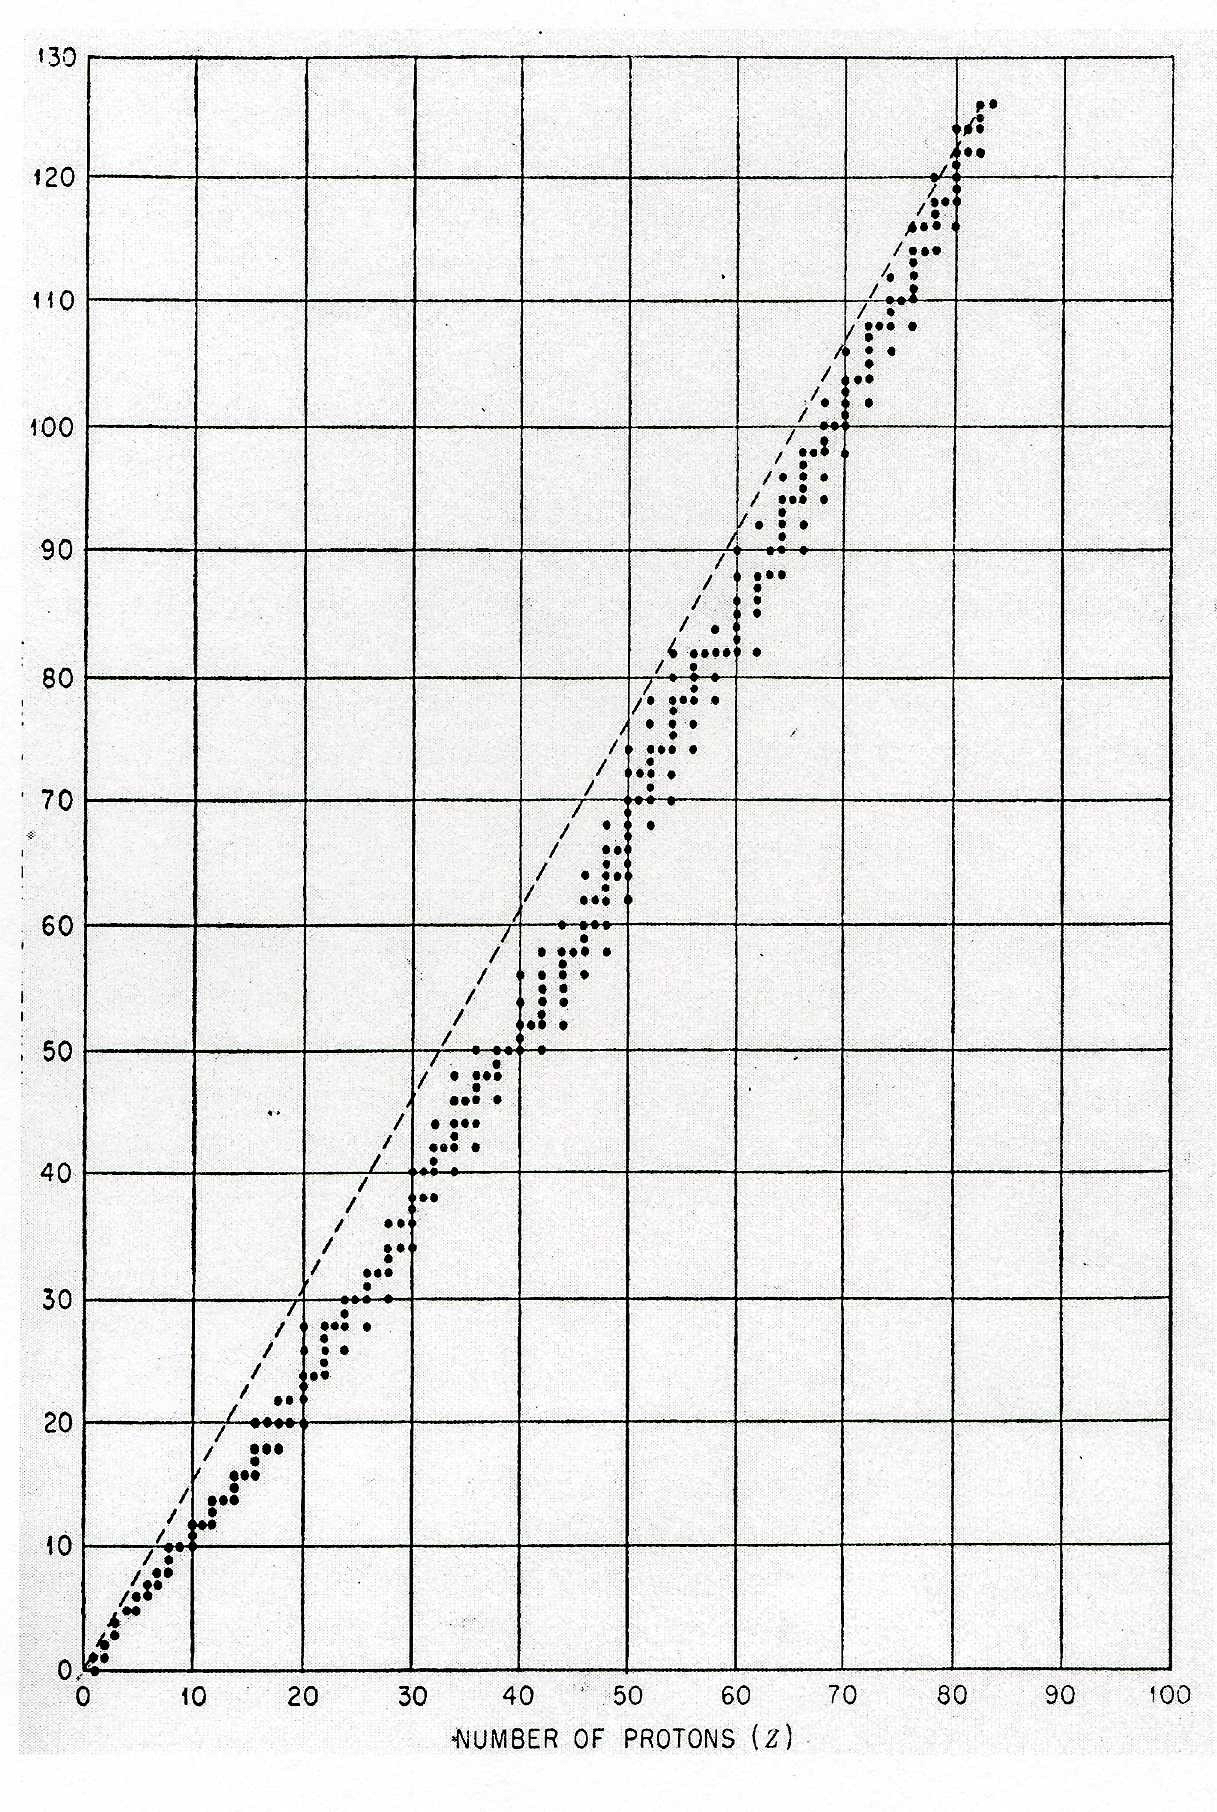
\includegraphics[scale=0.13]{ch1/image1.png}
	\captionof{figure}{ }
	\end{wrapfigure}
La stabilité des noyaux lourd est assurée par un excès du nombre de neutrons par rapport au 
nombre de protons. Le dernier élément stable est l'uranium $U$ ($Z=92$) que l'on trouve 
principalement en deux isotopes
\begin{enumerate}
\item $ ^{238}U$ $\approx$ 99.3\%
\item $ ^{235}U$ $\approx$ 0.7\%
\item $ ^{234}U$ $\approx$ traces
\end{enumerate}
Lorsque l'on observe la valée de la stabilité, on peut en effet voir que plus le nombre de 
proton augmente, plus le nombre de neutron fait de même pour stabiliser le noyau. Si un 
noyau doit se fissionner, il y aura un trop pleins de neutrons et ces derniers peuvent 
être réutiliser à certaines fins.\\ 
\\


	\begin{wrapfigure}[8]{r}{3.4cm}
	\vspace{-8mm}
	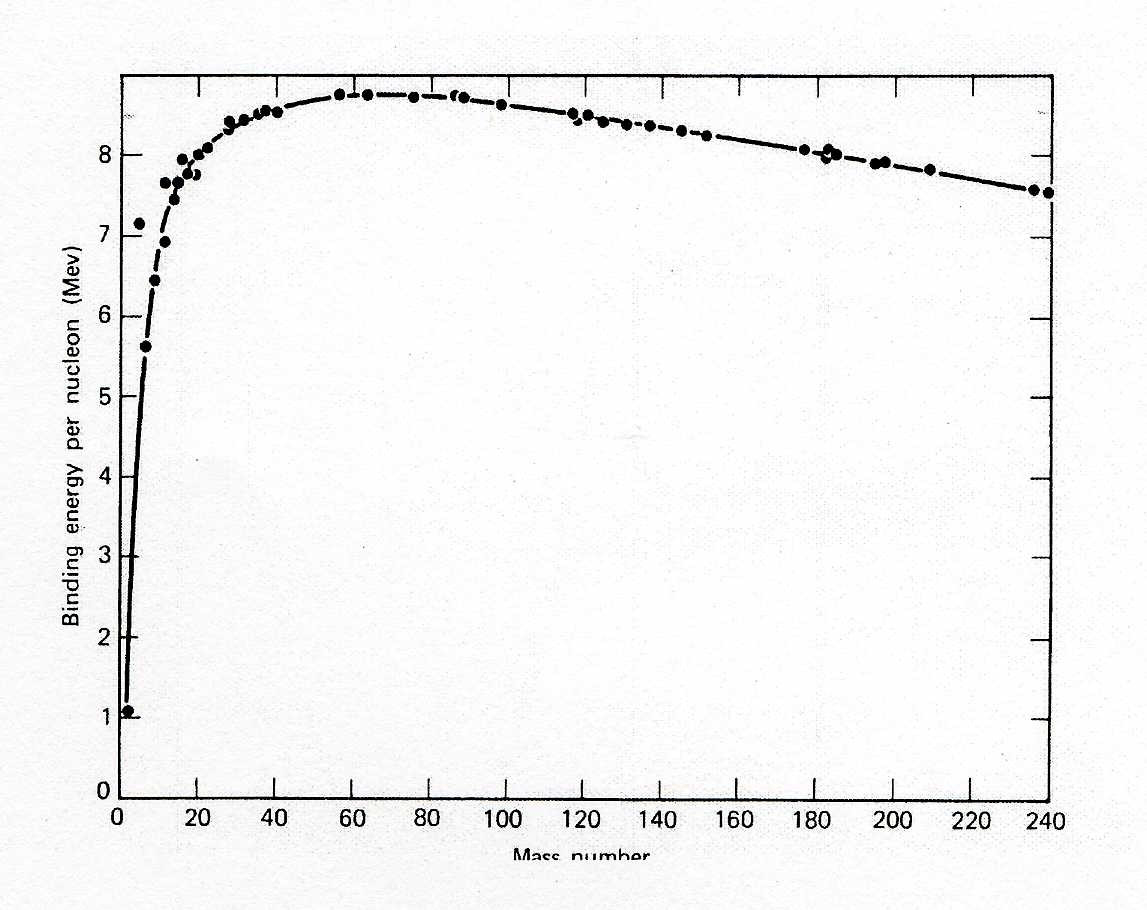
\includegraphics[scale=0.13]{ch1/image2.png}
	\captionof{figure}{ }
	\end{wrapfigure}
Une autre courbe connue est celle de l'\textit{énergie de liaison des noyaux}. Les noyaux 
possèdent un défaut de masse : la somme des masses des nucléons est plus élevée que la 
masse du noyau qu'ils constituent. Il en résulte forcéement une énergie qui a permis de 
réaliser cette liaison et c'est ce que reprend cette courbe : elle exprime cette énergie 
en fonction du nombre de masse.\\

Il existe alors deux façons de récupérer de l'énergie sur le défaut de masse. Soit en allant 
vers des noyaux qui ont un défaut de masse et récupérer cette énergie soit en fissionnant 
des noyaux lourds. 

\subsubsection{Isotopes fissiles et fertiles}
La nature n'offre pas des centaines de possibilités pour récupérer cette énergie liée au 
défaut de masse par fission : ces isotopes sont dit \textbf{fissiles} ($U_{235}$ (naturel), 
$U_{233}, Pu_{235}$. Par contre, d'autres sont dit \textbf{fertiles} : par capture neutronique, 
ils donnent lieu à un isotope fissile
\begin{equation}
\begin{array}{llll}
U_{238} + n\quad&\to\quad U_{239}+\gamma\quad&\overset{\underset{\Longrightarrow}{\text{23'}}}{\beta^-}\quad Np_{239}\quad&\overset{\underset{\Longrightarrow}{\text{2.3j}}}{\beta^-}\quad Pu_{239}
\vspace{2mm}\\
Th_{232} + n\quad&\to\quad Th_{233}+\gamma\quad&\overset{\underset{\Longrightarrow}{\text{22'}}}{\beta^-}\quad Pa_{233}\quad&\overset{\underset{\Longrightarrow}{\text{27.4j}}}{\beta^-}\quad U_{233}
\end{array}
\end{equation}
L'isotope le plus abondant de l'uranium est l'$U_{238}$ qui est forcément souvent présent dans 
les réacteurs : par ajout d'un neutron  et suite aux désintégrations $\beta$ il est possible de
créer du $Pu_{239}$ qui est fissile et s'ajoute ainsi à la matière fissile du réacteur. Hélas, 
$Pu_{239}$ est traiter comme un déchet, il n'est pas possible de l'utiliser\dots\\

De même, le thorium 232 est aussi susceptible de capturer un neutron et donner de l'uranium 233 par 
double désintégration $\beta$. On peut remarquer que les isotopes impair sont fissiles alors que les
fertiles sont pairs.\\

Le principal souci est l'abondance naturelle de $U_{235}$, seulement 0.7\%. On va alors utiliser 
de l'uranium enrichi. Pour que le réacteur fonctionne, il faudra un rapport $V/S$ choisi judicieusement afin d'éviter les fuites neutroniques et garantir une réaction en chaîne. Notons 
que l'enrichissement lié à la production d'électricité est de l'ordre que 3-4\% et de l'ordre de
plus de 90\% pour une bombe atomique.

\subsubsection{Énergie de fission}
La combustion d'un atome de carbone fourni une énergie de $3eV$ alors que la fission d'un noyau 
d'$U_{235}$ fourni 200 MeV, l'énergie susceptible d'être libérée est donc pharamineuse par rapport 
aux centrales thermiques. A partir d'un gramme d'$U_{235}$ (si fissionné entièrement) il est possible 
de fournir  1 MW durant une journée : seulement 3 kg d'$U_{235}$ sont suffisant pour faire tourner 
une centrale comme Doel 2 toute une journée.\\

Hélas, le cycle thermodynamique n'a qu'un rendement de 33\%. On distingue alors la \textit{puissance 
thermique} qui est l'énergie produite par le racteur par unité de temps (MWth) et la \textit{
puissance électrique} qui est la sortie du générateur (MWe).


\subsection{Interaction neutrons - noyaux lourds}
\subsubsection{Phénomènes possible}
Il existe plusieurs phénomènes possibles, en voici trois
\begin{enumerate}
\item \textit{Scattering}\footnote{Le scattering (diffusion) est le phénomène par lequel un rayonnement, comme la lumière, le son ou un faisceau de particules, est dévié dans diverses directions par une interaction avec d'autres objets.} du aux collisions : élastique (toute l'énergie est conservée) ou inélastique.
\item \textit{Fission}
\begin{center}
$U_{25}$ + $n$\quad$\to$\quad 2 fragments + $\gamma n + \beta + \gamma$
\end{center}
où $\nu$ est ne nombre de neutrons par fission.
\item \textit{Capture radiative}. Permet par exemple le passage de fertile à fissile
\begin{center}
$U_{25} + n\quad\to\quad U_{26}+\gamma$
\end{center}
\end{enumerate}



\subsubsection{Section efficace}
La \textbf{section efficace macroscopique} $\Sigma\ [cm^{-1}]$ est la probabilité \textbf{par unité de 
longueur\footnote{D'où le \textit{section}}} de rencontrer un type d'interaction  particulier 
dans un libre parcours dans un milieu donné. Dès lors $\Sigma$ est fonction du milieu, de 
l'énergie du neutron, de la position spatiale et, forcement, du type d'interaction.

Par exemple $\Sigma_t$ est la probabilité par unité de longueur de libre parcours 
d'avoir une interaction, quelque soit sa nature.
\begin{center}
\begin{tabular}{|c|c|}
\hline 
\multicolumn{2}{|c|}{Section efficaces en physique des réacteurs} \\ 
\hline 
\hline 
$\Sigma_{in}$ & Scattering inélastique \\ 
\hline 
$\Sigma_e$ & Scattering élastique \\ 
\hline 
$\Sigma_s = \Sigma_e+\Sigma_{in}$ & Scattering total \\ 
\hline 
$\Sigma_f$ & Fission \\ 
\hline 
$\Sigma_c$ & Capture photon $\gamma$ \\ 
\hline 
$\Sigma_a=\Sigma_c+\Sigma_f$ & Absorption (capture + fission) \\ 
\hline 
$\Sigma_t=\Sigma_a+\Sigma_s$ & Toutes les interactions \\ 
\hline 
\end{tabular} 
\end{center}


Le nombre de neutrons au bout d'un libre parcours sont ceux qui étaient déjà la moins ceux qui 
ne le sont plus
\begin{equation}
n(x+dx) = n(x)- \Sigma_t n(x) dx\quad \Leftrightarrow\quad \frac{n(x)}{n(0)} = e^{-\int_0^x \Sigma_t(x')dx'} \equiv pdf
\end{equation}
où $pdf$ signifie \textit{proba density function} (pour le libre parcours).\\

La probabilité d'une interaction dépend du nombre de noyau que l'on peut rencontrer. Il faut donc 
que la section efficace dépende de la densité atomique $[cm^{-3}]$
\begin{equation}
\Sigma = N.\sigma
\end{equation}
où $N=f(p,T)$ est la densité isotropique et $\sigma = f(noyau,\vec{v})$ la section efficace 
microscopique $[cm^2]$ qui dépend du mouvement relatif.\\


	\begin{wrapfigure}[11]{r}{4cm}
	\vspace{-8mm}
	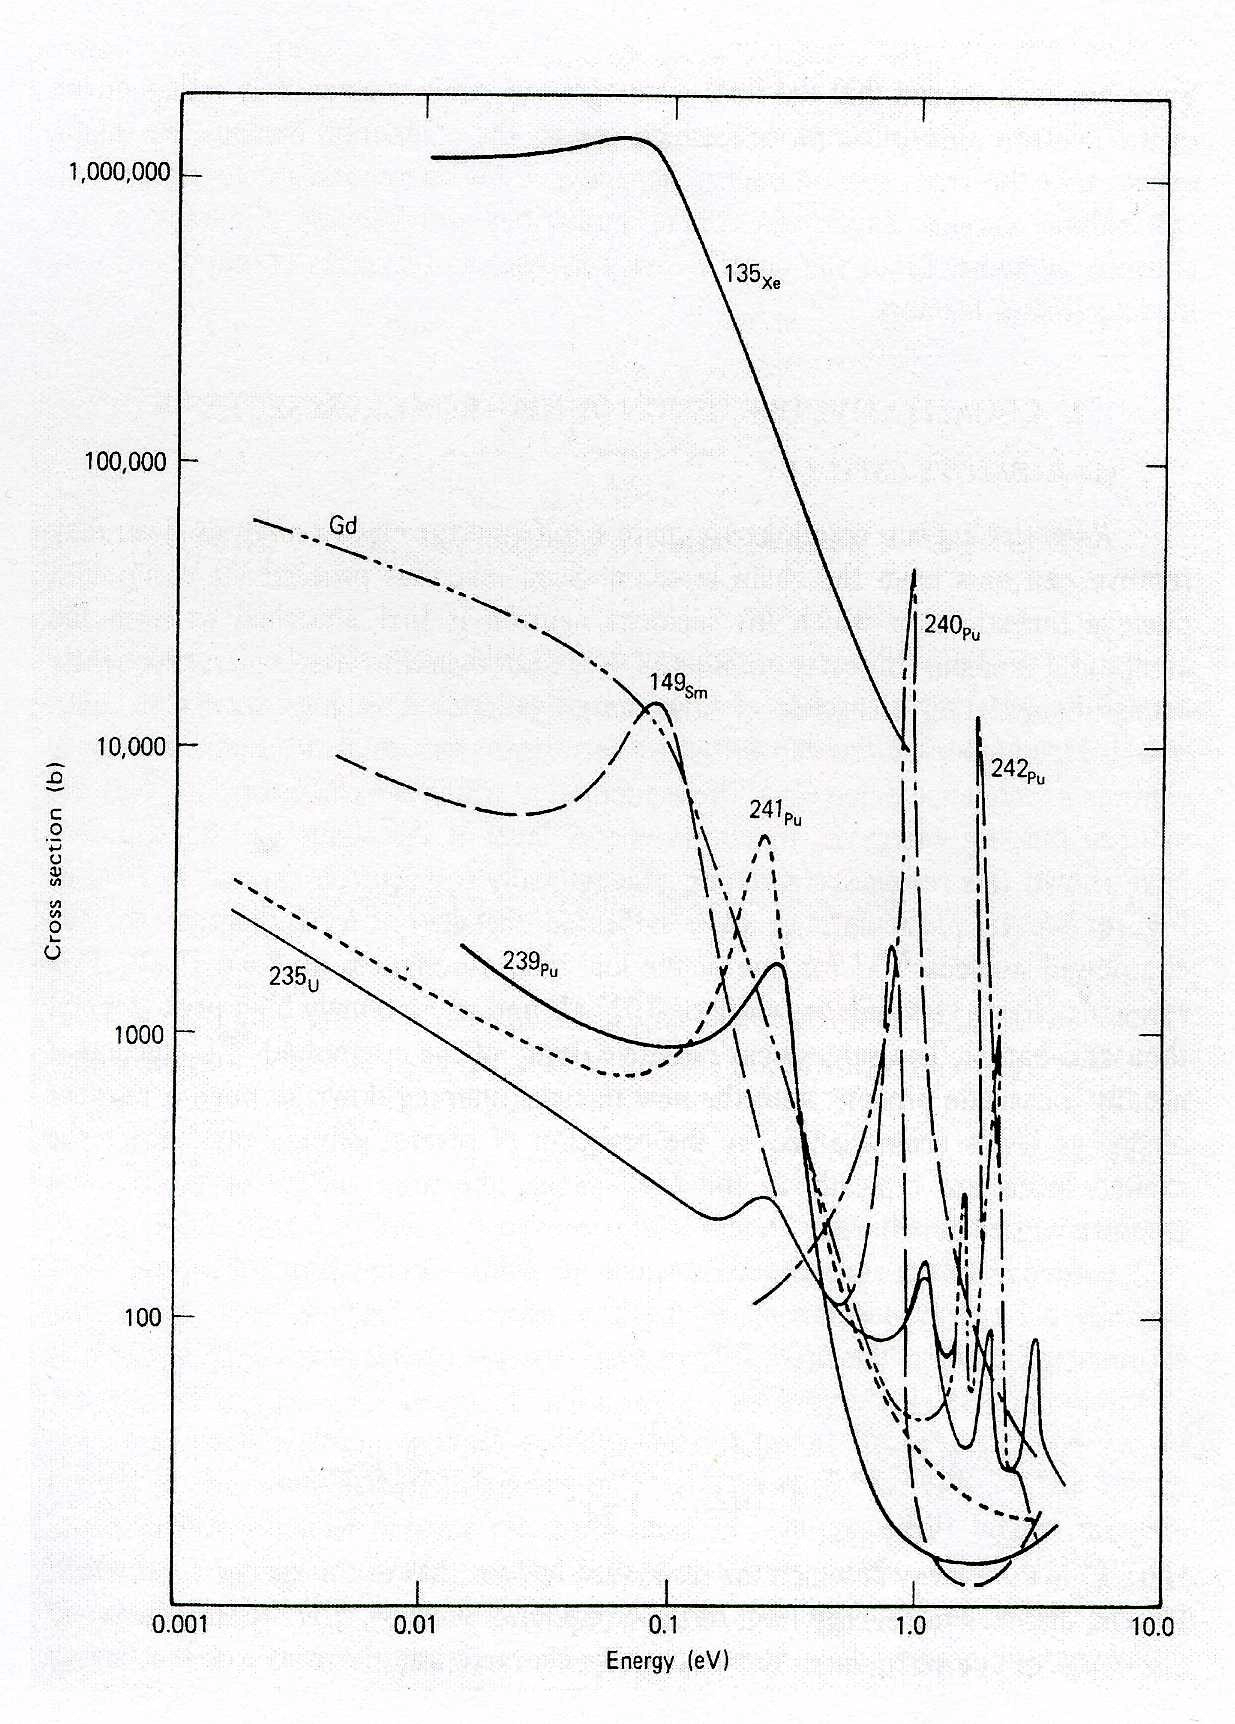
\includegraphics[scale=0.13]{ch1/image3.png}
	\captionof{figure}{ }
	\end{wrapfigure}
La section efficace est ici la section transverse (attention, même expression pour les deux en 
anglais même lorsqu'elles ne sont pas égales). On peut voir une section efficace comme un disque 
de probabilité qui peut grandir ou diminuer en fonction de la probabilité d'avoir interaction. C'est 
une notion qui remplace quelque part la section transverse géométrique.\\

Historiquement ; on imagine un neutron qui arrive face à une porte de grange (\textit{barn}) 
devant lui. On utilise alors cette unité plus adaptée : $1\ barn : 10^{-24}\ cm^2$. La section 
efficace dépend de l'énergie et l'écart entre deux phénomènes (fission et thermique) peut être 
de 8 décades.\\

Le graphique de la section efficace en fonction de l'énergie est un peu chaotique. A une température 
équivalent d'$\frac{1}{40}eV$ on retrouve des pics (résonance) : on ne parle plus de capture, 
fission, \dots \ mais de section efficace totale.\\

Regardons la gamme d'énergie que l'on peut rencontrer sur un réacteur. Un neutron émis par 
fission a une énergie d'environ 2 MeV. Or, ceci correspond à une section efficace diminuée de 
trois ordre de grandeur de ce que l'on pourrait aux énergies thermiques. Si on souhaite avoir 
de nouvelles fissions avec ces neutrons émis, il serait judicieux de les amener dans la zone 
thermique "à gauche" afin d'éviter la résonance.

\begin{center}
	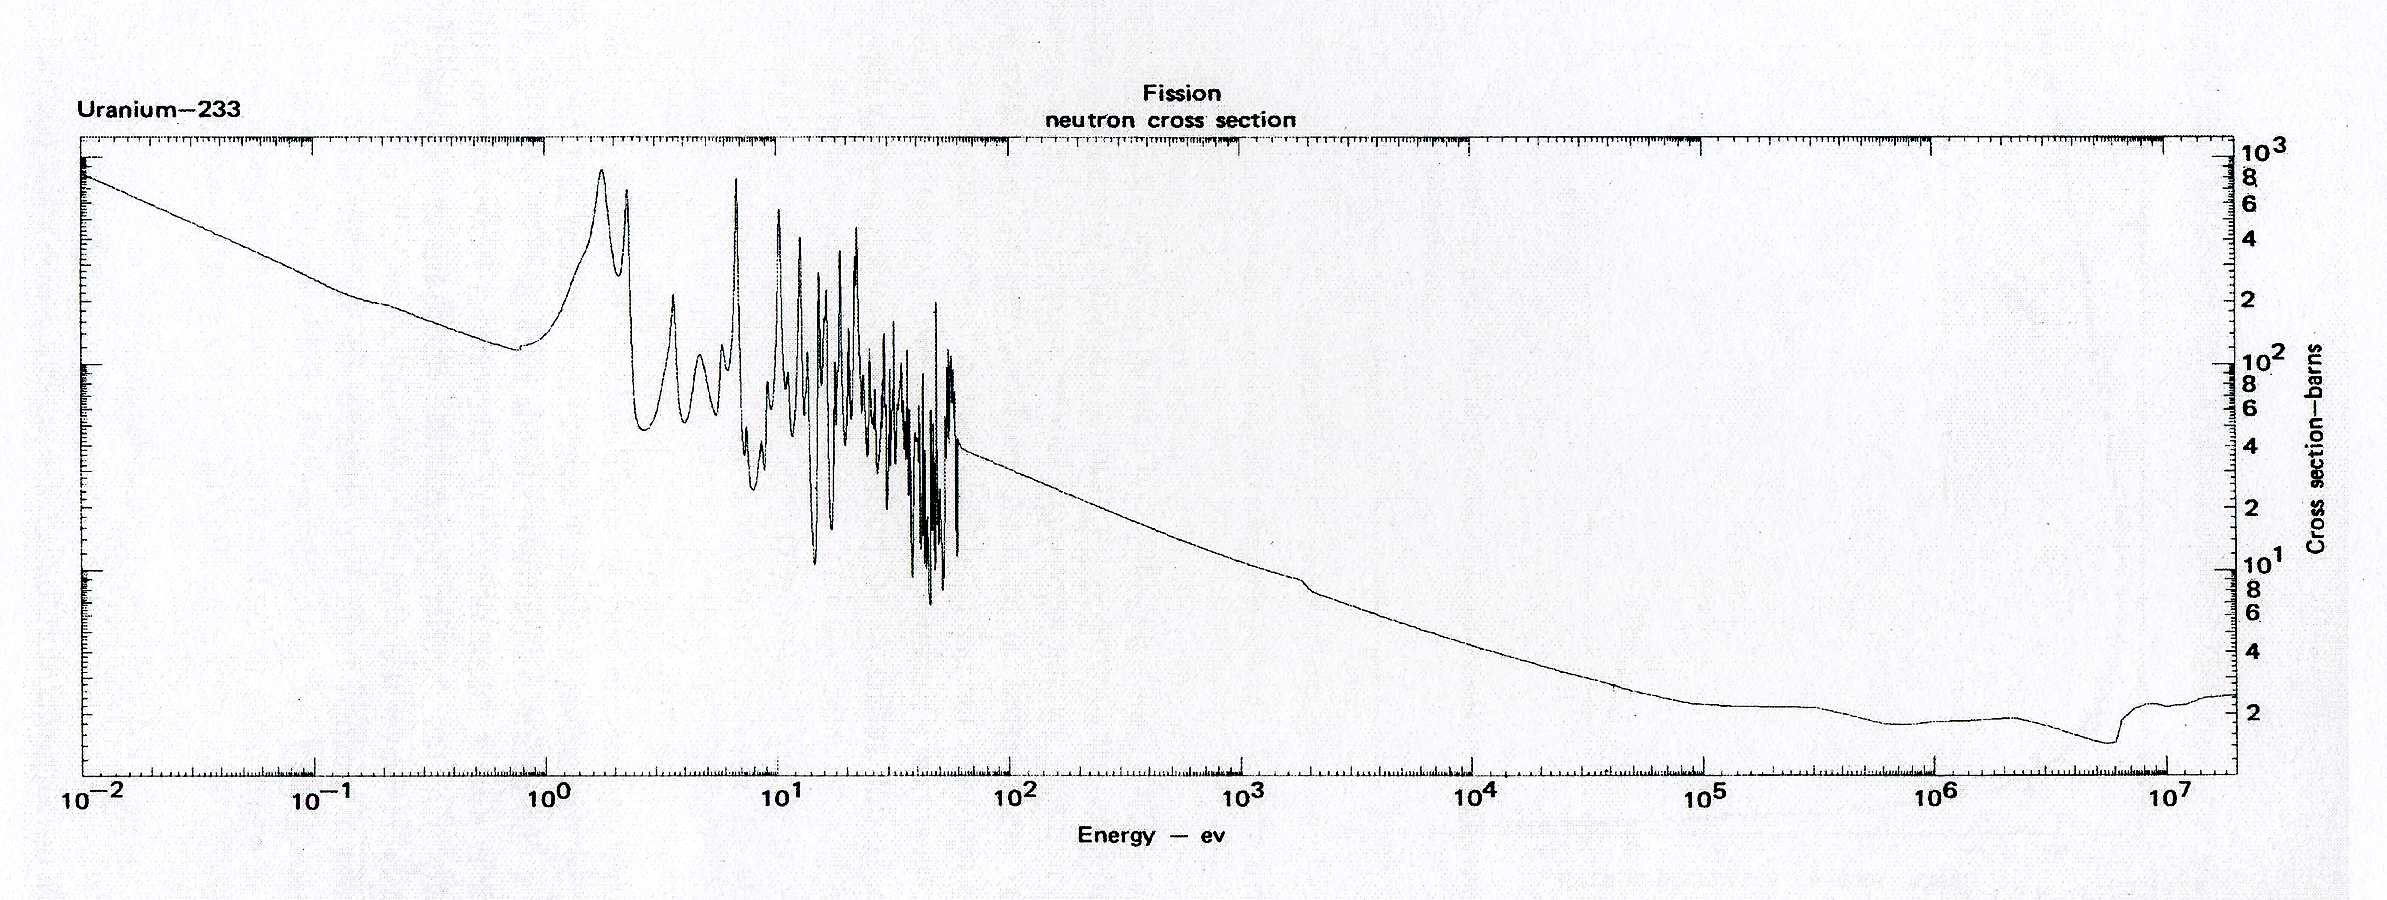
\includegraphics[scale=0.23]{ch1/image4.png}
	\captionof{figure}{ }
\end{center}

Les section efficace en terme de fission ; quand on se retrouve à l'énergie que les électrons ont après une fission, la section efficace des principaux isotopes fissibles sont 3 ordres de grandeur plus basse de ce qu'on peut avoir aux énergies thermiques. Il faut donc les refroidir suffisamment 
vite afin d'éviter qu'ils se retrouvent dans la zone dangereuse et y être mangé.\\


Pour les ralentir, il faudrait que les neutrons rentrent en collisions avec une autre "masse", de masse semblable de sorte à avoir un choc élastique. Une masse équivalent au neutron est le proton, 
on va alors utiliser l'eau (fluide caloporteur) qui va également jouer le rôle de ralentisseur de 
neutron pour un réacteur thermique afin qu'il soit suffisamment ralenti (et donc avec moins 
d'énergie) pour se trouver "a gauche" des résonance lors de sa collision avec un noyau lourd. On 
parle de \textit{neutrons thermiques}



\begin{center}
	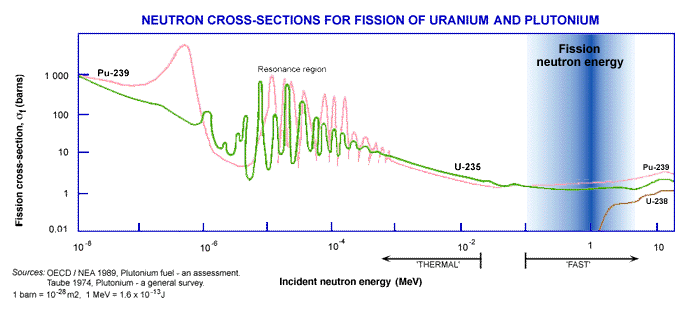
\includegraphics[scale=0.7]{ch1/image5.png}
	\captionof{figure}{ }
\end{center}

Il existe tout de même une petite marge pour tout de même faire autre chose : maintenir les énergies 
assez élevée afin de produire plus de matière fissile que ce qui a été consommé. En effet, si on 
parvient à légèrement monter les énergies il sera possible de fissionner l'$U_{238}$ qui produira 
de la nouvelle matière fissile, le $Pu_{239}$. On parle de \textit{neutrons rapides}. Pour les 
accélérer il ne faut pas utiliser de l'eau mais des éléments lourds.



\subsection{Cycle neutronique et criticité}
\subsubsection{Caractéristique d'un cycle}
	\begin{wrapfigure}[7]{r}{4cm}
	\vspace{-5mm}
	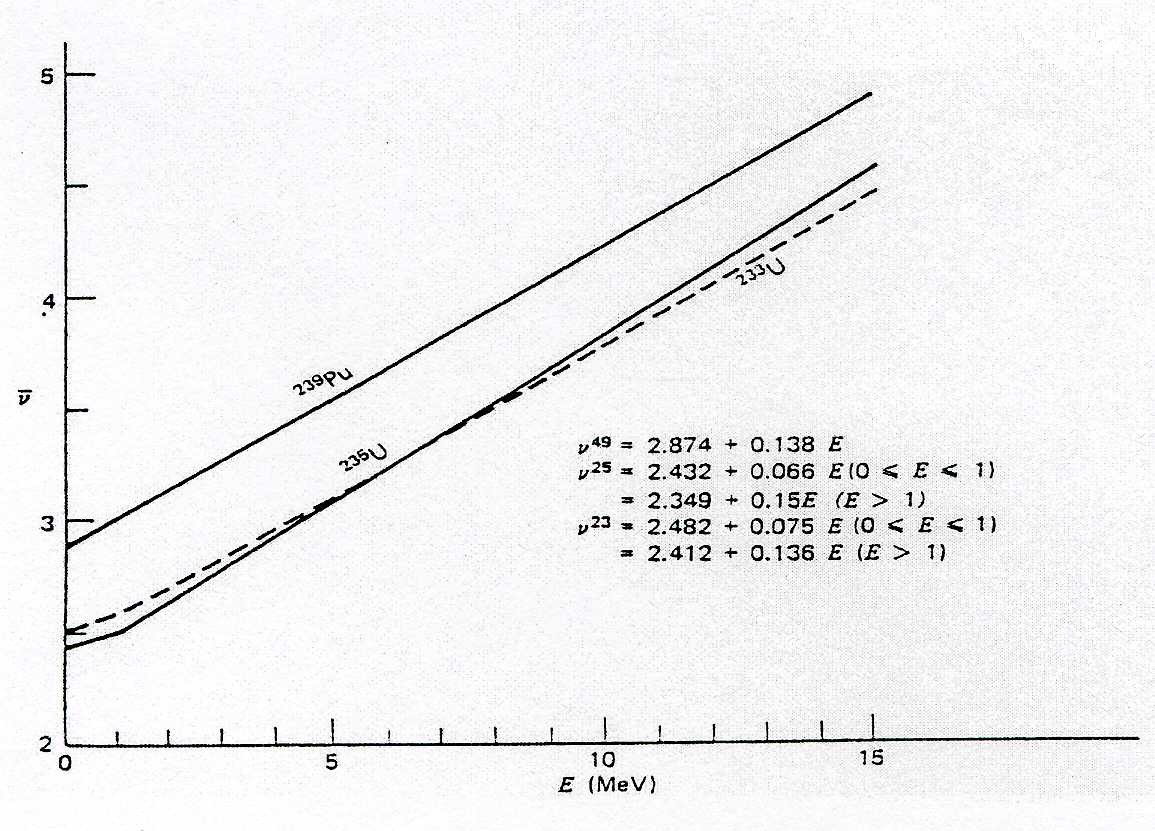
\includegraphics[scale=0.13]{ch1/image6.png}
	\captionof{figure}{ }
	\end{wrapfigure}
On souhaiterait avoir une réaction auto-entretenue. Pour se faire, on est en possession du nombre 
moyen de neutrons émis par fission. Pour l'$U_{235}$
\begin{equation}
\nu(E) = \left\{\begin{array}{ll}
2.432 +0.66E&\quad E\geq 1\\
2.349+0.15E&\quad E>1
\end{array}\right.
\end{equation}

\subsubsection{Paramètre de régénération}
Un autre paramètre souvent introduit est $\eta$. La différence par rapport à $\nu$ est qu'il 
s'agit d'une absorption. On exprime $\eta$ en multipliant le nombre de neutron moyen émis par
fission par la probabilité d'avoir une fission (donc la probabilité qu'un neutrons produit par 
fission donne lieu à une nouvelle fission) et l'on divise le tout par le nombre de neutrons
absorbés: c'est le \textbf{paramètre de régénération}
\begin{equation}
\eta = \dfrac{\text{Nb $n$ produced in the fuel}}{\text{Nb $n$ absorbed in the fuel}}\quad\Rightarrow
\quad \eta = \dfrac{\nu\sigma_f}{\sigma_f+\sigma_c}=\dfrac{\nu}{1+\alpha}
\end{equation}
où $\alpha = \sigma_c/\sigma_f$. Ce paramètre dépend fortement de l'énergie. Si il y a plusieurs 
isotopes, il faut tenir compte des densités isotropiques (la section efficace macroscopique donne
le nombre moyen pondéré)
\begin{equation}
\eta = \dfrac{\sum_j\nu_j\Sigma_{fj}}{\sum_j \left(\Sigma_{fj}+\Sigma_{cj}\right)}
\end{equation}


\subsubsection{Breeding ratio (taux de reproduction)}
Ce ratio est lié au fait qu'il y a un excès de neutrons par rapport à ce qui est consommé : si l'on 
fait le bilan, on obtient chaque fois un nombre supplémentaire. Si $F$ est la fraction de ces 
neutrons qui vont être absorbés par le matériau fertile pour donner naissance à l'isotope associé, 
on définit le \textbf{breeding ration}
On le définit comme
\begin{equation}
BR = (\eta-1)F
\end{equation}
où $\eta-1$ est l'excès de neutrons disponible pour la reproduction.\\

\textsc{Criticité}\\
On parle de \textit{criticité} lorsque le réacteur peut fonctionner de façon stationnaire sans 
qu'il y ait apport extérieur de neutron : ce-dernier produit tous les neutrons nécessaire. Cet 
équilibre 1/1 dépend d'une configuration générale du réacteur. Un réacteur critique est donc 
une condition d'équilibre qui n'a \textbf{rien} à voir avec la puissance.

\newpage
Afin de savoir si l'on est à la criticité, on introduit le facteur de réacteur $k$ qui est 
le nombre moyen de neutrons émis lors d'un cycle complet. Voyons comment exprimer ce facteur dans 
le cadre d'un réacteur infini. \\

	\begin{wrapfigure}[11]{r}{7.5cm}
	\vspace{-5mm}
	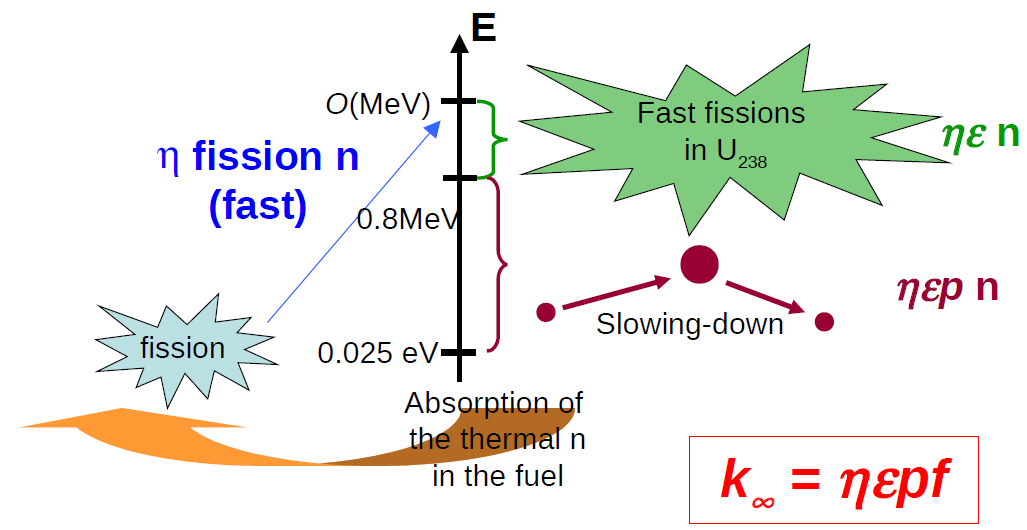
\includegraphics[scale=0.3]{ch1/image7.png}
	\captionof{figure}{ }
	\end{wrapfigure}
Partons d'un gentil petit neutron thermique (fraction d'eV) absorbé par le combustible. Combien 
de ces neutrons vont être émis ? C'est le fameux paramètre $\eta$. A partir d'un neutron, on a 
$\eta$ neutrons émis suite aux fissions. Une fraction $\epsilon$ de ces $\eta$ neutrons sont dans 
la gamme rapide et vont conduire à des fissions (et donc augmentation du nombre de neutrons). Ces
neutrons vont ensuite ralentir et doivent survivre à ce ralentissement : seulement une fraction 
$p$ (probabilité anti-trappe) survit. On a donc pour un neutron $\eta\epsilon p$ qui atteignent 
le domaine thermique et $f$ (facteur d'usage thermique) d'entre-eux sont absorbés par le combustible et "recommencer" le cycle. 
On obtient la \textit{formule des quatre facteurs}
\begin{equation}
k_\infty = \eta\epsilon  pf
\end{equation}

Ceci est pour le cas d'infini, mais dans un cas réel il va y avoir des fuites : $P_f$ est la 
probabilité de "ne pas fuir" au ralentissement et $P_{th}$ la probabilité de ne pas se barrer 
du réacteur en allant jusqu'aux énergies thermiques 
\begin{equation}
k_{eff} = k_\infty P_fP_{th} = \eta \varepsilon pfP_fP_{th}
\end{equation}

	\begin{wrapfigure}[11]{l}{7.5cm}
	\vspace{-5mm}
	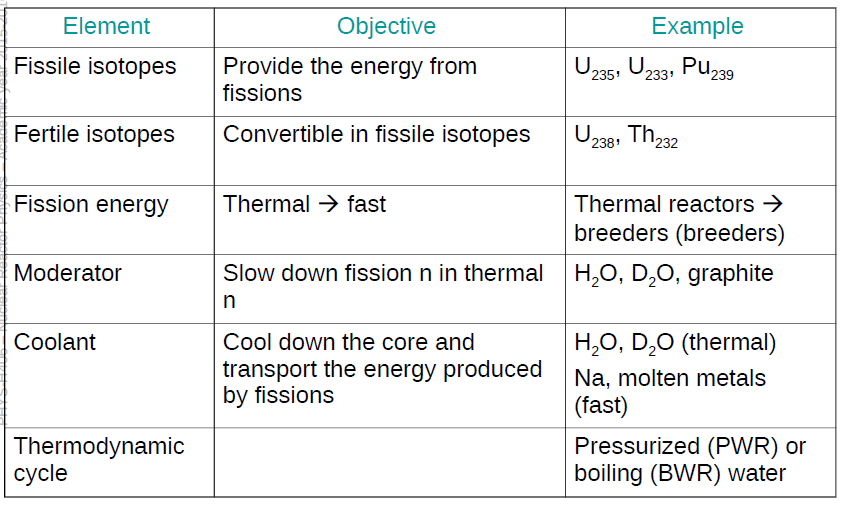
\includegraphics[scale=0.33]{ch1/image8.png}
	\captionof{figure}{ }
	\end{wrapfigure}
Comme $P_fP_{th} < 1$, il faut que $k_\infty > 1$. On pratique $1 \ll k_\infty$ car lorsque le 
réacteur tourne, il produit beaucoup de déchets. La capacité d'émettre des neutrons avec du 
combustible "frais" est plus importante en fin de cycle. Il peut donc y avoir un certain 
empoisonnement du réacteur. Tous ces facteurs $P,k_\infty$ dépendent de la géométrie et la 
nature des matériaux : il s'agit d'une balance entre la géométrie et les propriétés 
neutroniques\footnote{Si on souhaite faire monter la puissance d'un réacteur, il faut 
aller au delà de la criticité.}.\\


On a parle de survie aux fuites  mais un réacteur n'est pas dans un vide absolu. Quand un 
neutron quitte le réacteur on le reverra plus. Dans la réalité il serait pas mal d'utiliser 
un "réflecteur" : un matériau qui se trouve autour du combustible pour tenter de 
rétrodiffuser une partie de ces neutrons qui se font la maille. Ce n'est personne d'autre 
que l'eau qui joue ce rôle : l'eau a donc un rôle caloporteur, modérateur mais aussi réflecteur. \\

On définit la \textit{réactivité} comme la distance par rapport à la criticité. La protection 
majeure est l'utilisation de barres qui absorbe les neutrons. En cas d'arrêt d'urgence 
("\textit{scram}") ces barres sont plongées et le réacteur est au moins à l'arrêt malgré beaucoup de
chaleur émise.

\section{Profil de section efficaces}
\subsection{Mécanismes d'interactions}
Il faut que la gamme $\lambda$ des neutrons qui restent (dans l'énergie $E$ considérée) soit bien 
supérieur à la taille du noyau afin de pouvoir considérer une réaction du  noyau dans son ensemble
et non pas pour chacun de ses nucléons. Il se produit deux mécanismes
\begin{enumerate}
\item Potentiel de scattering : choc sans interactions avec la structure interne du noyau
\item Résonances : interaction avec la structure interne (désexcitation, constitution d'un noyau 
composé)
\end{enumerate}

\subsubsection{Énergie apportée par un neutron incident sur un noyau}
Considérons comme système de départ un neutron incident et un autre corps qui est un noyau $(A,Z)$
\begin{equation}
E_{tot} = m_{(A,Z)}c^2 + m_nc^2+E_{cin}
\end{equation}
Le second système est un noyau composé $(A+1, Z)$
\begin{equation}
E_{tot}=E_{tot} = m_{(A+1,Z)}c^2 +E_{cin}+\dots\ ? 
\end{equation}
Il y a donc un manque au niveau de l'énergie totale. Faisons un bilan en calculant l'énergie 
associé au défaut de masse du noyau ($B$ pour \textit{bind}, lier)
\begin{equation}
B(A,Z) = (A-Z)m_nc^2+Zm_pc^2 - m_{(A,Z)}c^2
\end{equation}
L'énergie pour séparer un neutron du noyau $(A+1,Z)$ :
\begin{equation}
S_n = B(A+1,Z)-B(A,Z) = m_nc^2+m_{(A,Z)}c^2-m_{(A+1,Z)}c^2
\end{equation}
C'est précisément ce qu'il nous manquait pour avoir conservation de l'énergie : il faut 
rajouter l'énergie de séparation.
\begin{equation}
E_{tot}=E_{tot} = m_{(A+1,Z)}c^2 +E_{cin}+S_n
\end{equation}
On peut voir cette "énergie de séparation" comme l'énergie qu'apporte "en plus" de son énergie 
cinétique un neutron. C'est une caractéristique non banale car on peut interpréter cette variation 
du défaut de masse comme le fait qu'une particule apporte en plus que son énergie cinétique une 
énergie un peu plus importante que la réalité du fondamental. 

\subsection{Sections efficaces associées}
\subsubsection{Capture $\gamma$}
	\begin{wrapfigure}[10]{l}{7.5cm}
	\vspace{-5mm}
	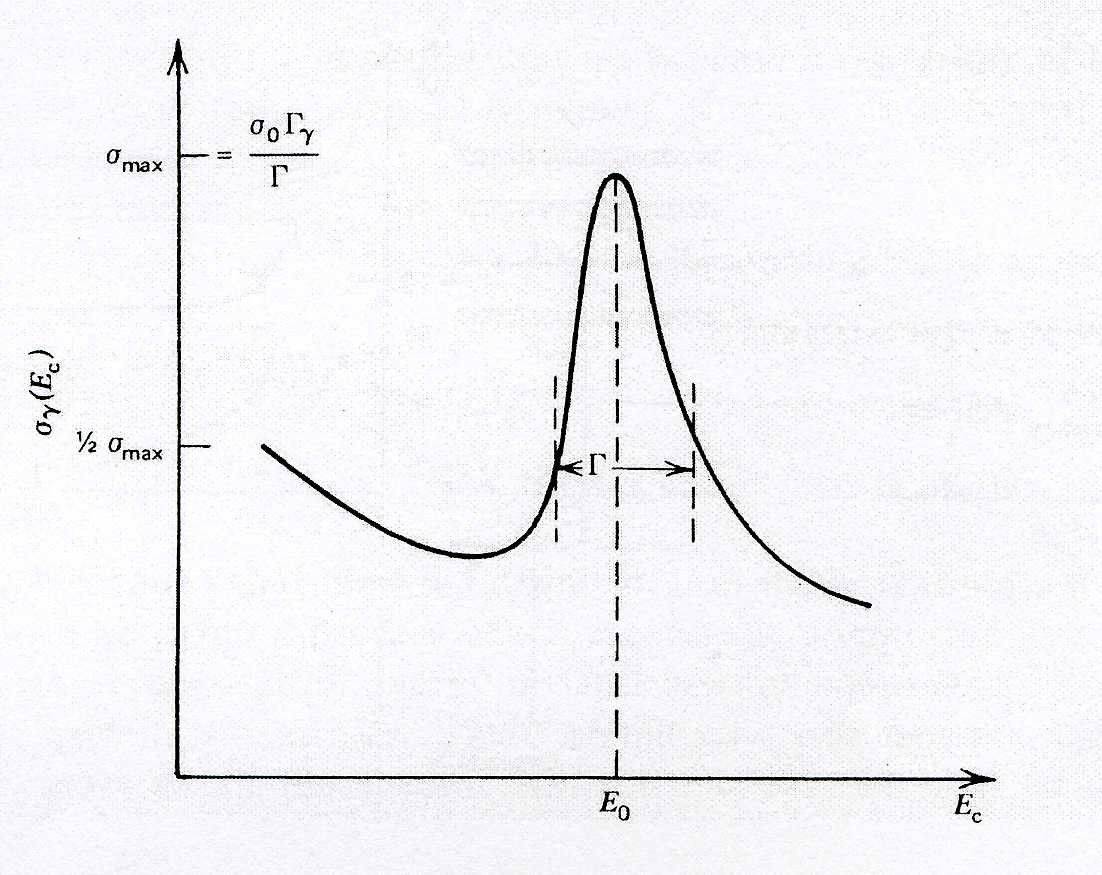
\includegraphics[scale=0.23]{ch1/image9.png}
	\captionof{figure}{ }
	\end{wrapfigure}
Il s'agit du modèle typique : un neutron est absorbé, il constitue un noyau composé qui se 
désexcite
\begin{center}
neutron absorbé $\longrightarrow$ noyau composé $\longrightarrow$ $\gamma$
\end{center}
Soit $\sigma_\gamma$ les résonance aux niveaux d'énergies $E$ du noyau composé. Il existe un 
modèle qui permet de modéliser la dépendance en énergie
\begin{equation}
{\sigma _\gamma } = \frac{\pi }{{{k^2}}}{g_J}\frac{{{\Gamma _n}{\Gamma _\gamma }}}{{{{(E - {E_o})}^2} + {\textstyle{{{\Gamma ^2}} \over 4}}}} \equiv {\sigma _o}\frac{{{\Gamma _\gamma }}}{\Gamma }\frac{1}{{1 + {x^2}}}
\end{equation}
où $x= \frac{E-E_0}{\gamma/2}$. On retrouve les largeur de raie $\gamma$ et un comportement en 
l'inverse de l'écart entre deux résonance. On peut même obtenir un comportement en $1/(1+x^2)$ si 
on utilise l'énergie \textit{relative} de la demi-largeur de raie. On peut voir ci-contre que 
en dehors des pics, on retrouve une gentille décroissance hyperbolique. Plus l'énergie est élevée, 
plus on observe une décroissance.

\subsubsection{Scattering (diffusion)}
\textsc{Diffusion élastique}\\
Pour le potentiel de scattering élestique le neutron, plutôt que d'être capturé, est réémis avec 
une autre directement mais "la même" énergie (c'est dans le mouvement relatif entre le neutron 
et le noyau que l'énergie est conservé)
\begin{center}
neutron absorbé $\longrightarrow$ noyau composé $\longrightarrow$ neutron réémis à "la même" énergie
\end{center}
On définit $\sigma_s$ comme la section efficace équivalente à la capture dans la résonance, au 
potentiel de diffusion et aux interférences
\begin{equation}
{\sigma _s} = \frac{\pi }{{{k^2}}}{g_J}\frac{{{\Gamma _n}{\Gamma _\gamma }}}{{{{(E - {E_o})}^2} + {\textstyle{{{\Gamma ^2}} \over 4}}}} + \frac{{4\pi R}}{k}{g_J}\frac{{{\Gamma _n}(E - {E_o})}}{{{{(E - {E_o})}^2} + {\textstyle{{{\Gamma ^2}} \over 4}}}} + 4\pi {R^2}
\end{equation}
Le premier terme est une lorentzienne près du pic de résonance et un terme supplémentaire lié aux 
interférences. Le comportement en énergie est différent et il est important de s'en souvenir. \\

\textsc{Diffusion inélastique}\\
Ici, la perte d'énergie est compensée par l'émission d'un photon gamma (lors de la désexcitation 
du noyau)
\begin{center}
neutron absorbé $\longrightarrow$ noyau composé $\longrightarrow$ neutron réémis à $E<E_i$
\end{center}
Cette diffusion inélastique est nulle jusqu'à un certain seuil ($\approx 10\ keV$ pour les 
noyaux lourds, plus élevé pour les noyaux légers)\footnote{Voir note, qqch pas clair avec la 
raison pour laquelle l'inélastique convient pas.}. Comme l'énergie est trop faible, ce type de 
diffusion n'aura que des effets dont nous ne tiendrons pas compte. Il faut garder à l'esprit que 
l'on peut ralentir le neutron sens perte d'énergie car c'est le mouvement relatif entre noyau et 
neutron qui est la caractéristique du scattering : on les modère élastiquement.\\

\textsc{Fission}\\
Le modèle est simple
\begin{center}
neutron absorbé $\longrightarrow$ noyau composé $\longrightarrow$ neutron réémis \dots
\end{center}
\dots + une désexcitation du noyau par fragmentaton en deux (ou trois) noyaux plus léger. Il 
peut exister un seuil (si non : fissile).




\newpage
\section{Fission nucléaire}
\subsection{Description}
Essayons de retrouver les éléments qui constituent ce phénomène de fission. Séparons l'énergie de 
séparation d'un neutron
\begin{equation}
{S_n} = B(A,Z) - B(A - 1,Z)  {\kern 1pt} {\kern 1pt}  = \frac{{B(A,Z)}}{A} + (A - 1).
\underbrace{\left( {\frac{{B(A,Z)}}{A} - \frac{{B(A - 1,Z)}}{{A - 1}}} \right)}_{<0}
\end{equation}
L'énergie $S_n$ est inférieur à l'énergie de liaison $E$ par nucléon pour un noyau lourd mais 
$S_n$ est le minimum d'énergie pour passer d'un noyau $(A-1,Z)$ à un noyau composé $(A,Z)$.

\subsubsection{Semi-empirique formule pour la masse d'un noyau}
En première approximation, l'énergie de liaison est proportionnel au nombre de masse. Ceci implique 
que 
$$m(\text{noyau}) \propto A$$
Le rayon d'un noyau est donné par $R=r_0.\sqrt[3]{A}$ impliquant que
$$V(\text{noyau}) \propto A$$
En supposant une densité +/- constante et que le noyau se comporte comme un liquide incompressible, 
on peut utiliser la formule semi-empirique de Weizsäcker
\begin{equation}
B(A,Z) = {a_v}A - {a_s}{A^{2/3}} - {a_a}\frac{{{{(A - 2Z)}^2}}}{A} - {a_c}\frac{{{Z^2}}}{{{A^{1/3}}}} + \delta (A,Z)
\end{equation}
où le premier terme est du à la tension superficielle, le second à l'asymétrie $N-Z$, le troisième 
à la répulsion coulombienne et le dernier est un facteur de parité de spin : ce terme est dominant 
pour les noyaux lourds
\begin{equation}
\delta(A,Z) = \left\{\begin{array}{ll}
\frac{a_p}{A^{3/4}} & Z, N\ \text{pairs}\\
\frac{a_p}{A^{3/4}} & A\ \text{impair}\\
-\frac{a_p}{A^{3/4}} & Z, N\ \text{impairs}
\end{array}\right.
\end{equation}
Dans un cas l'énergie de liaison augmente et dans l'autre pas
\begin{enumerate}
\item Noyau (Z pair, N impair) $\to$ Noyau (Z pair, N pair) $\Rightarrow +a_p/A^{3/4}$
\item Noyau (Z pair, N pair) $\to$ Noyau (Z pair, N impair) $\Rightarrow -a_p/A^{3/4}$
\end{enumerate}
Il en résulte une différence de $S_n = 2a_p/A^{3/4}$ soit de l'ordre du MeV! On voit donc 
que si on fissioner avec un neutron thermique il faut lui adjoindre une énergie cinétique 
de quasi 1 MeV pour compenser cette énergie\footnote{C'est le seuil d'énergie à fournir 
pour rendre un matériau fertile fissile.}. 



\subsubsection{Fission spontanée v.s. induite}
\subsubsection{Capture $\gamma$}
	\begin{wrapfigure}[14]{l}{7.5cm}
%	\vspace{-5mm}
	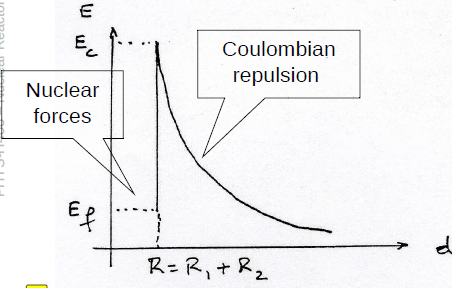
\includegraphics[scale=0.6]{ch1/image10.png}
	\captionof{figure}{ }
	\end{wrapfigure}
Soit une réaction de fission
\begin{equation}
(A,Z) \to (A_1,Z_1)+(A_2,Z_2)
\end{equation}
La masse du noyau initial est supérieur à celle des fragments. Est-il possible de voir un tel 
phénomène apparaître de façon spontanée ? Oui, mais pas observée. L'énergie potentielle des 
fragments es tune fonction de la distance entre eux :$E_c$ l'énergie du potentiel de Coulomb, $d
=R_1+R_2$ la distance entre les charges $Z_1,Z_2$, $E_f$ la différence d'énergie de liaison entre 
$(A,Z)$ et ses fragments. Les noyaux sont "un peu" trop gros pour l'effet tunnel. \\

	\begin{wrapfigure}[14]{r}{7.5cm}
	\vspace{-5mm}
	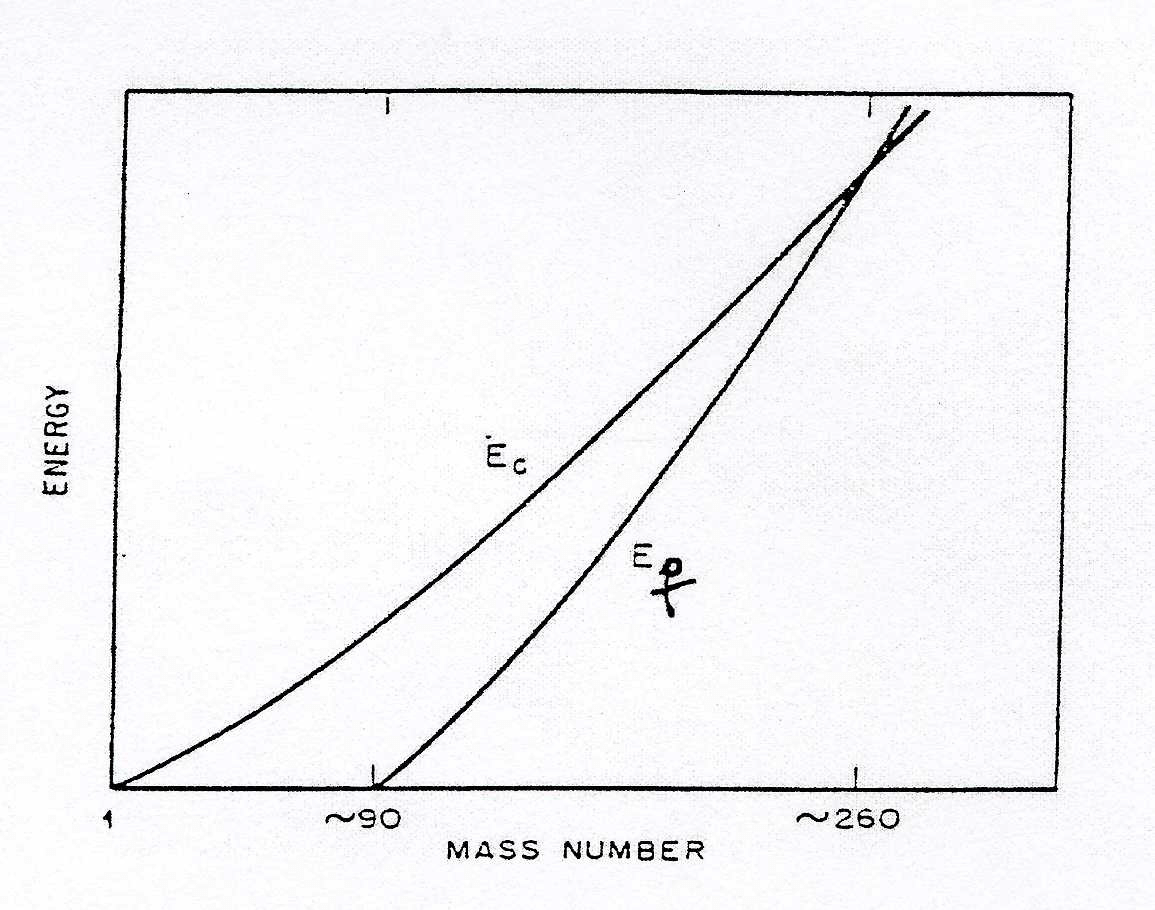
\includegraphics[scale=0.25]{ch1/image11.png}
	\captionof{figure}{ }
	\end{wrapfigure}
L'énergie permettant la fission est apportée par le neutron ($S_n+E_{cin}$) pour compléter 
$E_c-E_f$ (différence d'énergie entre coulomb et fission). Prenons par exemple la fission 
symétrique. Des que l'on dépasse 260 comme nombre de masse, il n 'y a plus d'équilibre. Dans 
l'intervalle qui nous intéresse $A\in[230,240]$, la différence entre la hauteur de la barrière 
coulombienne et le fond du puits est de $E_c-E_f=6$ MeV et l'énergie de liaison amenée par 
le neutron est du même ordre de grandeur $S_n = 6$ MeV. Avec cette énergie apportée on est à 
la hauteur de la barrière à franchir, il suffit d'un petit surplus d'énergie qui est apporté 
par l'énergie cinétique : la fission induite est possible.\\


\subsubsection{Développement d'une fission induite (capture $(n,f)$)}
Le temps d'absorption pour traverser un noyau est de $10^{-17}s$ alors que le temps de vie d'un 
noyau excité est de $10^{-14}$s ce qui est court, mais long par rapport au temps 
d'absorption d'un neutron : le système "a le temps" d'oublier les caractéristiques du neutron 
indicent. Il n'y a donc pas de raison d'avoir une distribution anisotrope, toutes les directions 
sont probables.\\

Par agitation des nucléons dans le noyau excité il se forme deux noyaux qui se font éjecter par 
la répulsion coulombienne en $10^{-20}$s. Comme on casse un noyau lourd, ces fragments ont un 
excédent de neutrons et sont hors équilibres. Pour se stabiliser, ils émettent directement 
($10^{-17}$s) des neutrons dit \textbf{prompts} : spectre isotrope donné par Maxwell
\begin{equation}
\chi (E) = \frac{2}{\theta }\sqrt {\frac{E}{{\pi \theta }}} .{e^{ - \frac{E}{\theta }}}
\end{equation}

Malgré ces émissions de neutrons, les fragments ne sont pas totalement désexcité et émettent 
des $\gamma$ (prompt, $10^{-14}s$) sur des temps courts. L'énergie cinétique des fragments 
reprend une grande partie des 200 MeV disponibles. Ces fragments, produits de fissions, sont 
parti pour des désintégrations $\beta$ car déficit de protons présent.


\subsection{Neutrons retardés}
Les produits de fissions cherchent toujours à se désexciter quelque peu (souvent l'émission 
de $\gamma$) mais parfois (si $E_{excit}$ suffisant) ils font office d'émetteur de neutrons 
\textbf{retardés} : émet des neutrons lors de la désintégration mais beaucoup plus tardivement 
que les prompts (les producteurs de neutrons retardés sont les \textbf{précurseurs}).

\subsubsection{Évolution de la population de neutrons $N$}
Soit $N$ le nombre de neutrons et $k$ la durée moyenne d'un cycle qui vaut $\approx 10^{-4}$s
\begin{equation}
\frac{dN}{dt} = \dfrac{k_{eff}-1}{l}N\quad\Leftrightarrow\quad N(t)=N(0)e^{\frac{k_{eff}-1}{l}t}
\end{equation}
Pour $N$ neutrons présent par cycle $l$, on produit $k_eff-1$(1= celui que l'on a envoyé) neutrons.
Si $k_{eff}=1.001$ on trouve
\begin{equation}
\frac{N(1s)}{N(0)} \approx e^{10}\ !!!
\end{equation}
Toute petite modification conduit a une augmentation de la population neutronique immense ! 
Heureusement, la réalité est différentes car les temps caractéristiques sont beaucoup plus long 
grâce aux neutrons retardés\footnote{On a joute au $(1-\beta)l\approx 10^{-4}$ les temps de vie 
des neutrons retardés}
\begin{equation}
l \longrightarrow (1-\beta)l + \sum_i\beta_iT_i \approx 10^{-1}\ s
\end{equation}
Si $k_{eff}=1.001$ on trouve
\begin{equation}
\frac{N(1s)}{N(0)} \approx e^{0.01}
\end{equation}
Cette variation est tout à fait gérable. En conclusion, l'émission de neutrons retardés par les
précurseurs n'est peut-être que de 0.68\% mais c'est la clef pour le contrôle du réacteur car 
sans eux il n'y a rien qui peut s'opposer à une variation de l'ordre de $e^{10}$.